\chapter{Technisches Konzept}

\section{Verwendete Frameworks}

\begin{table}[!ht]
    \centering
    \begin{tabular}{|l|l|} 
    \hline
    \textbf{NestJS}                                                                       & \textbf{ExpressJS}                                                                    \\ 
    \hline
    \emph{NodeJS Framwork}                                                              & \emph{NodeJS Framework}                                                             \\ 
    \hline
    + Durch vorgegebene Struktur lässt sich das Projekt eher strukturiert halten & - Projekt wird bei großer Projektgröße schnell unstrukturiert                \\ 
    \hline
    + Durch die strukturierte Arbeitsweise gut für Teams geeignet                & - Durch die Freiheit bei Technologiewahl eher für einzelne Developer besser  \\ 
    \hline
    - weniger Freiheit bei Implementation                                        & + Mehr Freiheit bei der Implementation durch weniger Strukturvorgaben        \\ 
    \hline
    - Aufgrund strengerer Strukturvorgaben schwerer zu lernen                    & + Durch einfachen Aufbau leicht zu erlernen                                  \\ 
    \hline
    - relativ neue Technologie mit weniger Nutzern                               & + Viele Nutzer und dadurch auch viel Dokumentation                           \\
    \hline
    \end{tabular}
    \end{table}

NestJS war eine Vorgabe des Product Owners (IT Designers Gruppe) für die Entwicklung einer Back-End API. 
Es ist ein Framework das auf der JavaScript Umgebung NodeJS aufbaut und den Code in Module, Controller und Services aufteilt und somit eine klare Struktur zur Entwicklung vorgibt.\\
Aufgrund diesen strengen Strukturvorgaben, sind NestJS Anwendungen, im Vergleich mit bspw. ExpressJS, sehr gut skalierbar.

\begin{table}[!h]
    \centering
    \begin{tabular}{|l|l|} 
    \hline
    \textbf{React}                                                                      & \textbf{Angular}                                                                    \\ 
    \hline
    \emph{JS Library}                                                             & \emph{JS Library}                                                           \\ 
    \hline
    + Vorbereitung für Praxissemester (Wird mind. 1 Teammitglied sicher verwenden) & - Nicht sicher im Praxissemester verwendet                \\ 
    \hline
    + Sehr einfaches erstellen von GUIs                & - Erstellen von Benutzeroberflächen etwas komplizierter  \\ 
    \hline
    - weniger strukturiert                                        & + Schon sehr ähnlich zu NestJS strukturiert        \\ 
    \hline
    + mehr Freiheit bei Implementation                    & - weniger Freiheit bei Implementation                                  \\ 
    \hline
    - aufgrund weniger Strukturvorgaben schwerer große Projekte sauber zu halten                               & + aufgrund der erzwungenen Struktur ergeben sich auch bei großen Projekten wenig Probleme                           \\
    \hline
    \end{tabular}
    \end{table}

Einige unserer Teammitglieder haben vor, im Praktikumssemester React zu nutzen. 
Außerdem ist React im Vergleich zu Angular noch etwas einfacher zu lernen.
Daher fiel auch die Wahl auf React, trotz der sehr NestJS-ähnlichen Struktur die Angular bietet.


\begin{table}[!h]
    \centering
    \begin{tabular}{|l|l|} 
    \hline
    \textbf{MongoDB}                                                                      & \textbf{MySQL}                                                                    \\ 
    \hline
    + No SQL Datenbank & - SQL Datenbank               \\ 
    \hline
    + Datenstrukturen sind näher an tatsächlicher Implementation                & - Datenstrukturen sind abstrakt, nicht so nah an der Implementation  \\ 
    \hline
    + Speichert Daten im JSON Format => Struktur nah an Objekten                                        & - Speichert Daten in Tabellen        \\ 
    \hline
    - Für uns neue Technologie                   & + Schon bekannt aus vorherigen Semestern                                  \\ 
    \hline
    \end{tabular}
    \end{table}

Auch MongoDB war eine Vorgabe des ProductOwners.
Im Vergleich zu “klassischen” Datenbanken wie MySQL halten MongoDB Datenbanken ihre Daten nicht in Tabellen, sondern in JSON Files in einer Baumstruktur, d.h. MongoDB ist eine sog. NoSQL Datenbank. \\
Daher ist MongoDB im vergleich zu bspw. MySQL Datenbanken schon von der Grundstruktur der Datenhaltung sehr nah an der tatsächlich in der Entwicklung genutzten Strukturen der Implementation und verlangt so weniger Abstraktion als eine SQL Datenbank.
\pagebreak
\section{Softwarearchitektur}

\begin{figure}[!h]
    \centering
    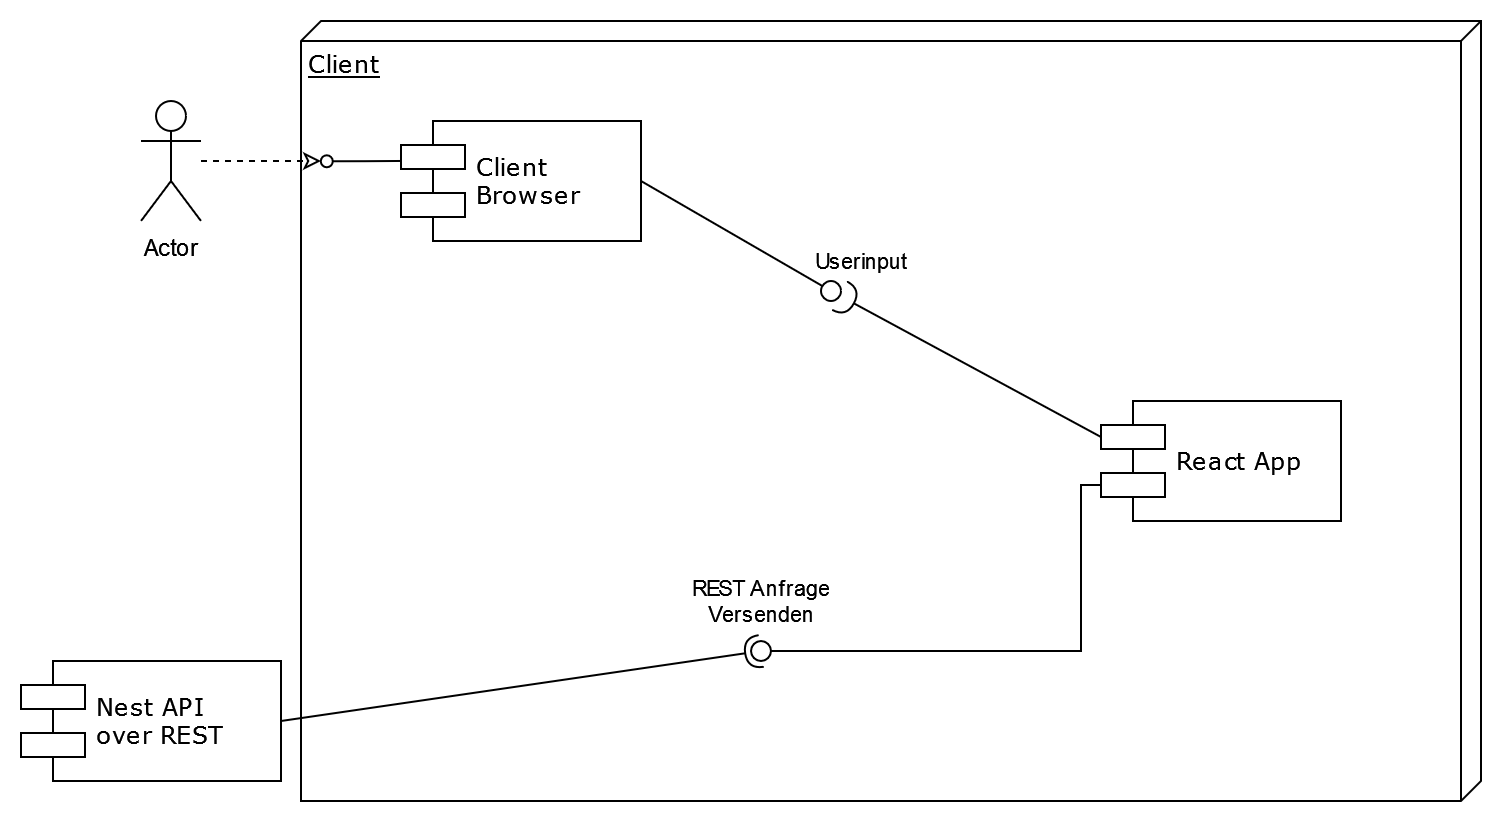
\includegraphics[width=0.8\textwidth]{./UML_Diagrams/ComponentDiagramClient.png}
    \caption{Component Diagram: Client}
    \label{fig:ComponentDiagramClient}
\end{figure}
In Abbildung 4.1 ist das Komponentendiagramm des Client zu sehen.
Dieses beschreibt die verwendeten Komponenten bei eingegangenem User Input.
Der Nutzer macht über den Web-Client eine Anfrage, wie beispielsweise der Aufruf der Web-Applikation oder die Anfrage auf einen bestimmten Raum.
Dadurch fordert der Client ein Interface über die React App, welche dann eine REST Anfrage an die Nest API schickt.
Im Normalfall sollte dann die REST Anfrage beantwortet werden und die React App kann mit den erhaltenen Informationen ein geeignetes User Interface zur Nutzung auf dem Client bereitstellen.

\begin{figure}[!h]
    \centering
    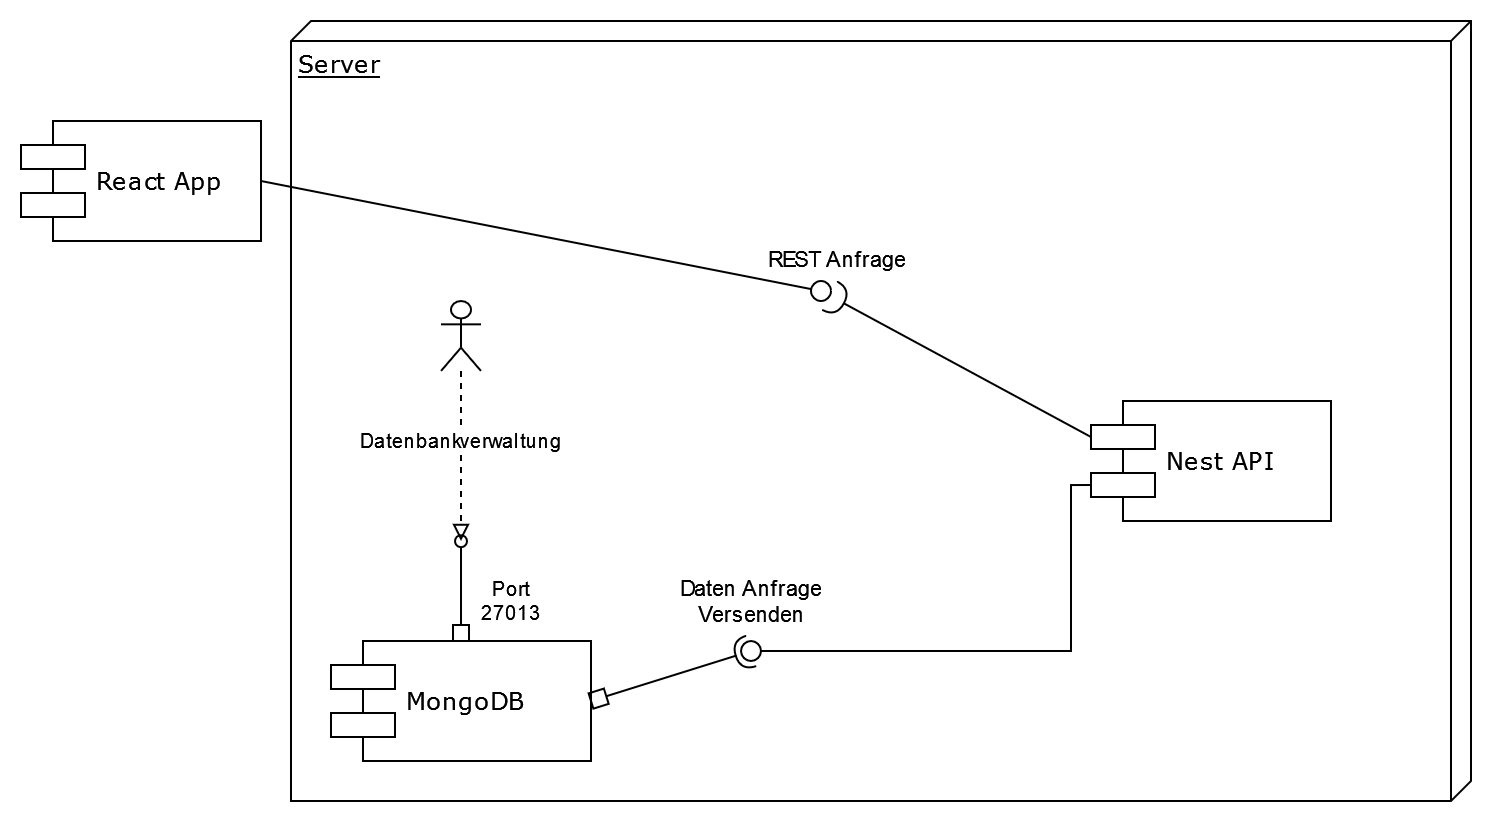
\includegraphics[width=0.8\textwidth]{./UML_Diagrams/ComponentDiagramServer.png}
    \caption{Component Diagram: Server}
    \label{fig:ComponentDiagramServer}
\end{figure}
In Abbildung 4.2 ist das Komponentendiagramm des Servers zu sehen.
Dieses beschreibt die verwendeten Komponenten bei eingegangener REST Anfrage.
Die React App stellt eine REST Anfrage an die NEST API, diese fordert dann die verlangten Informationen über ein Interface von der Mongo Datenbank.
Die MongoDB ist erreichbar über den Port 27013 durch den Datenbank-Administrator, dieser bearbeitet die Anfrage und sendet die gefordeten Daten über das Interface zurück an die Nest API.
Zu guter Letzt kann die Nest API dann die bereitgestellten Informationen über ein geeignetes Interface an die React App schicken, welche dadurch weitere Anfragen, wie mithilfe des Komponentendiagramm des Clients beschrieben wurde, beantworten kann.



\begin{figure}[!h]
    \centering
    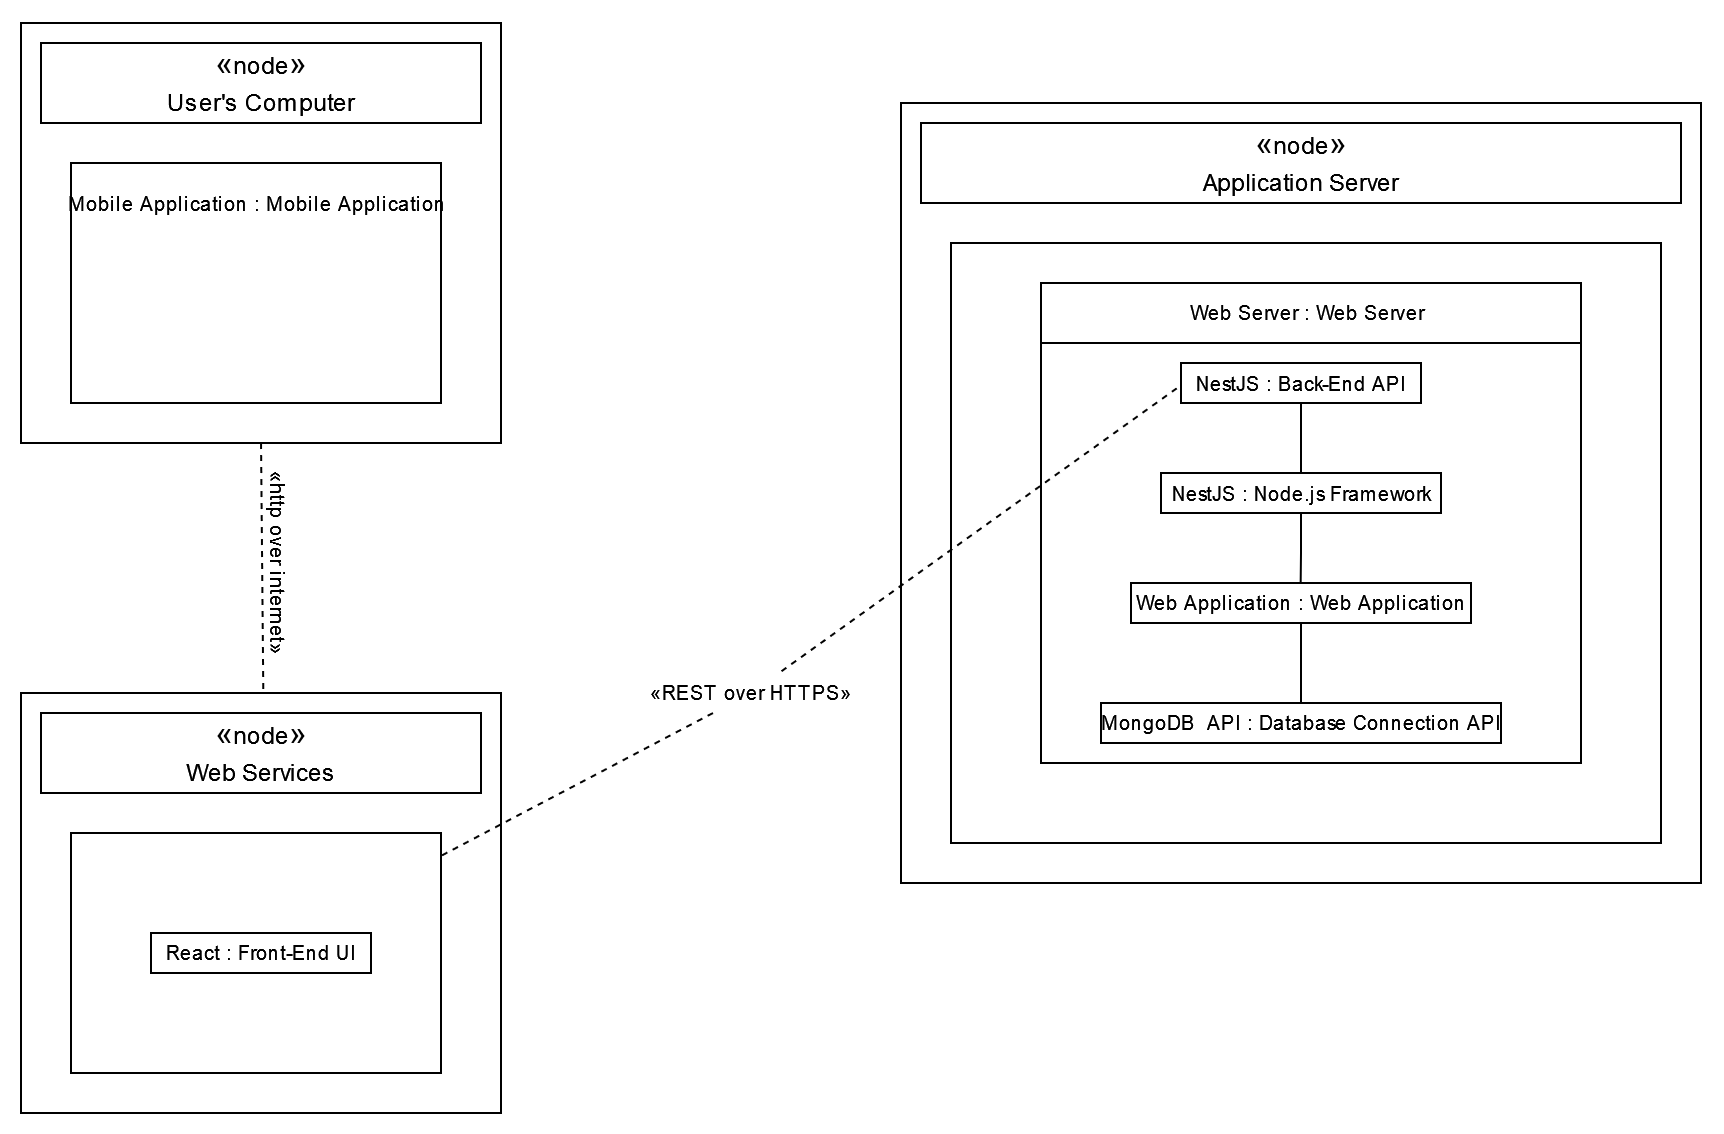
\includegraphics[width=0.8\textwidth]{./UML_Diagrams/Verteilungsdiagramm.png}
    \caption{Verteilungsdiagramm}
    \label{fig:Verteilungsdiagramm}
\end{figure}

Das in Abbildung 4.3 gezeigte Verteilungsdiagramm veranschaulicht, wie die Applikation im Browser des Nutzers über das React-Framework an das NestJS backend verbunden ist.
Der Nutzer sendet mithilfe der Benutzeroberflächen eine HTTP Anfrage an das React Front-End über das Internet, um zum Beispiel Informationen über Räume anzufordern.
Das React Front-End sendet die Anfrage des Nutzers mittels REST Anfrage über HTTPS an das NestJS Backend, damit dies an die Datenbank zugreifen kann.
Das NestJS Backend sendet die Anfrage an die Mongoose Datenbank und liefert die geforderten Informationen zurück.


\section{Datenbanken}